%\documentclass[12pt,draft]{IEEEtran} %!PN
\documentclass[12pt,journal,draftclsnofoot,onecolumn]{IEEEtran}
%\documentclass[12pt]{../springer/llncs}
%\usepackage{makeidx}  % allows for indexgeneration
%\documentclass[usletter,12pt]{report}
%\documentclass[usletter,12pt]{article}
\usepackage{latexsym}
\usepackage{amssymb}
\usepackage{amsbsy}
\usepackage{amsmath}
\usepackage{multirow}
\usepackage{listings} 
\usepackage{xcolor}
\lstset{ %numbers=left, 
	%numberstyle= \tiny, 
	keywordstyle=\color{blue},
	commentstyle=\color[cmyk]{1,0,1,0}, %设置注释颜色
	frame=single,
	breaklines,
	extendedchars=false,
	tabsize=4, %设置tab空格数
	showspaces=false %不显示空格
	%rulesepcolor= \color{ red!20!green!20!blue!20} 
} 
%\usepackage{subeqnarray}
%\usepackage[subnum]{cases}
\usepackage{longtable}
\usepackage{pifont}
\usepackage{times}
%\usepackage{fancybox}
\usepackage{graphicx}
\usepackage{subfigure}
%\includegraphics*[width=xx,height=yy]{filename}
\pagestyle{plain}
%\setlength{\parskip}{0.15in}
%\setlength{\oddsidemargin}{-.0in}
%\setlength{\textwidth}{6.5in}
%\setlength{\topmargin}{-0.0in}
%\setlength{\headheight}{0.0in}
%\setlength{\headsep}{0.0in}
%\setlength{\textheight}{8.3in}
%\setlength{\textheight}{8.5in}

\newcommand{\rmv}[1]{}
%\renewcommand{\baselinestretch}{1.6}
%\renewcommand{\thesection}{\Roman{section}.}
%\renewcommand{\thesection}{\arabic{section}}
%\renewcommand{\thesubsection}{\Alph{subsection}.}
%\renewcommand{\thesubsection}{\arabic{section}.\arabic{subsection}.}
%\renewcommand{\theequation}{\arabic{equation}}
%%\renewcommand{\theequation}{\arabic{section}.\arabic{equation}}
%\renewcommand{\thefigure}{\arabic{figure}}
%\renewcommand{\thetable}{\arabic{table}}
%\renewcommand{\thempfootnote}{\alph{footnote}}
%\renewcommand{\thempfootnote}{\fnsymbol{footnote}}

\newtheorem{theorem}{Theorem}
%\newtheorem{corollary}{Corollary}
\newtheorem{algorithm}{Algorithm}
%\newtheorem{definition}{Definition}
%\newtheorem{evaluation}{Evaluation}
\newtheorem{lemma}{Lemma}
\newtheorem{example}{Example}
\newtheorem{fact}{Fact}
%\newtheorem{property}{Property}

%\setcounter{page}{100}
\usepackage{url}
\usepackage{shorttoc}
\usepackage{color}

\begin{document}

%\mainmatter

\baselineskip=22 pt

\begin{titlepage}
\thispagestyle{empty}


\title{EE5414 Course Mini Project Report (BeagleBone Black)}

\author{\authorblockN{Wangchen DAI (53623708)}\\
\author{\authorblockN}{Jingwei HU (53656463)}\\
Instructor: Dr. L L CHENG\\
\authorblockA{Department  of Electronics Engineering\\
City University of Hong Kong}\\
\today}

\maketitle
\end{titlepage}

%\tableofcontents
\shorttableofcontents{Contents}{2}
\clearpage

\section{Introduction}\label{Intro}
An embedded system is a computer system with a specific function and embedded in a mechanical or electrical system. Due to the limitation of processing resurces, lower power consumption, smaller size, lower cost, and simpler operating function are the main properties of embedded computers when compared with the general ones. Embedded systems are usually based on microcontrollers or microprocessors, such as MCU, ARM, DSP and FPGA. In this project, an ARM based circuit board, BeagleBone Black (BBB), is applied as the hardware development tool. An Ubuntu14.04 terminal system, which is known as a kind of open source Linux system, is loaded into the ARM7 chip as the software development platform. Using this specified embedded system, a series of functions are developed including: LED Test, Image/Video Capture, Web Server and SQL Server Establishment.

% % % % % % % % % % % % % % % % % % % % % % % % % % % % % % % % %
% % % % % % % % % % % % % % % % % % % % % % % % % % % % % % % % %
\section{Hardware Description and Implementation}\label{HdDes}
BBB is a low-cost, community-supported hardware platform for embedded application development. BBB board mainly contains an ARM Cortex A8 series processor, a 512MB DDR3 RAM memory, an onboard 2GB MMC chip, and some other necessary peripherals. In this project, the BBB is developed with following cables and devices: \\
$\bullet$ A MiniUSB Cable, which can be used to connect the board with PC and served as power source (limited to 500mA), network, and serial port for data transmission;\\
$\bullet$ An external DC power supply with a minimum of 1A current output;\\
$\bullet$ An USB Hub to expand the onboard USB Host port from one to four;\\
$\bullet$ An USB portable 802.11N wireless adapter;\\
$\bullet$ A Logitech HD Pro C920 Web Camera, which is a USB webcam and provides full HD 1080p video recording in wide-screen at a maximum rate of 30 frames pre second;\\
$\bullet$ A mini SD card and its corresponding USB portable card reader.\\
The detailed and connection information of all hardware cables and devices is provided in both Fig.\ref{hw1}, for block diagram view, and Fig.\ref{hw2} for real view.
\begin{figure}[ht]
	\centering
	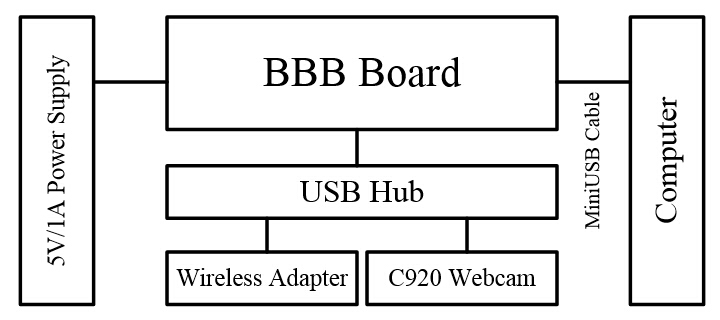
\includegraphics[width=4in]{./figs/hw1.jpg}
	\caption{Block diagram of hardware description.}
	\label{hw1}
\end{figure}
\begin{figure}[ht]
	\centering
	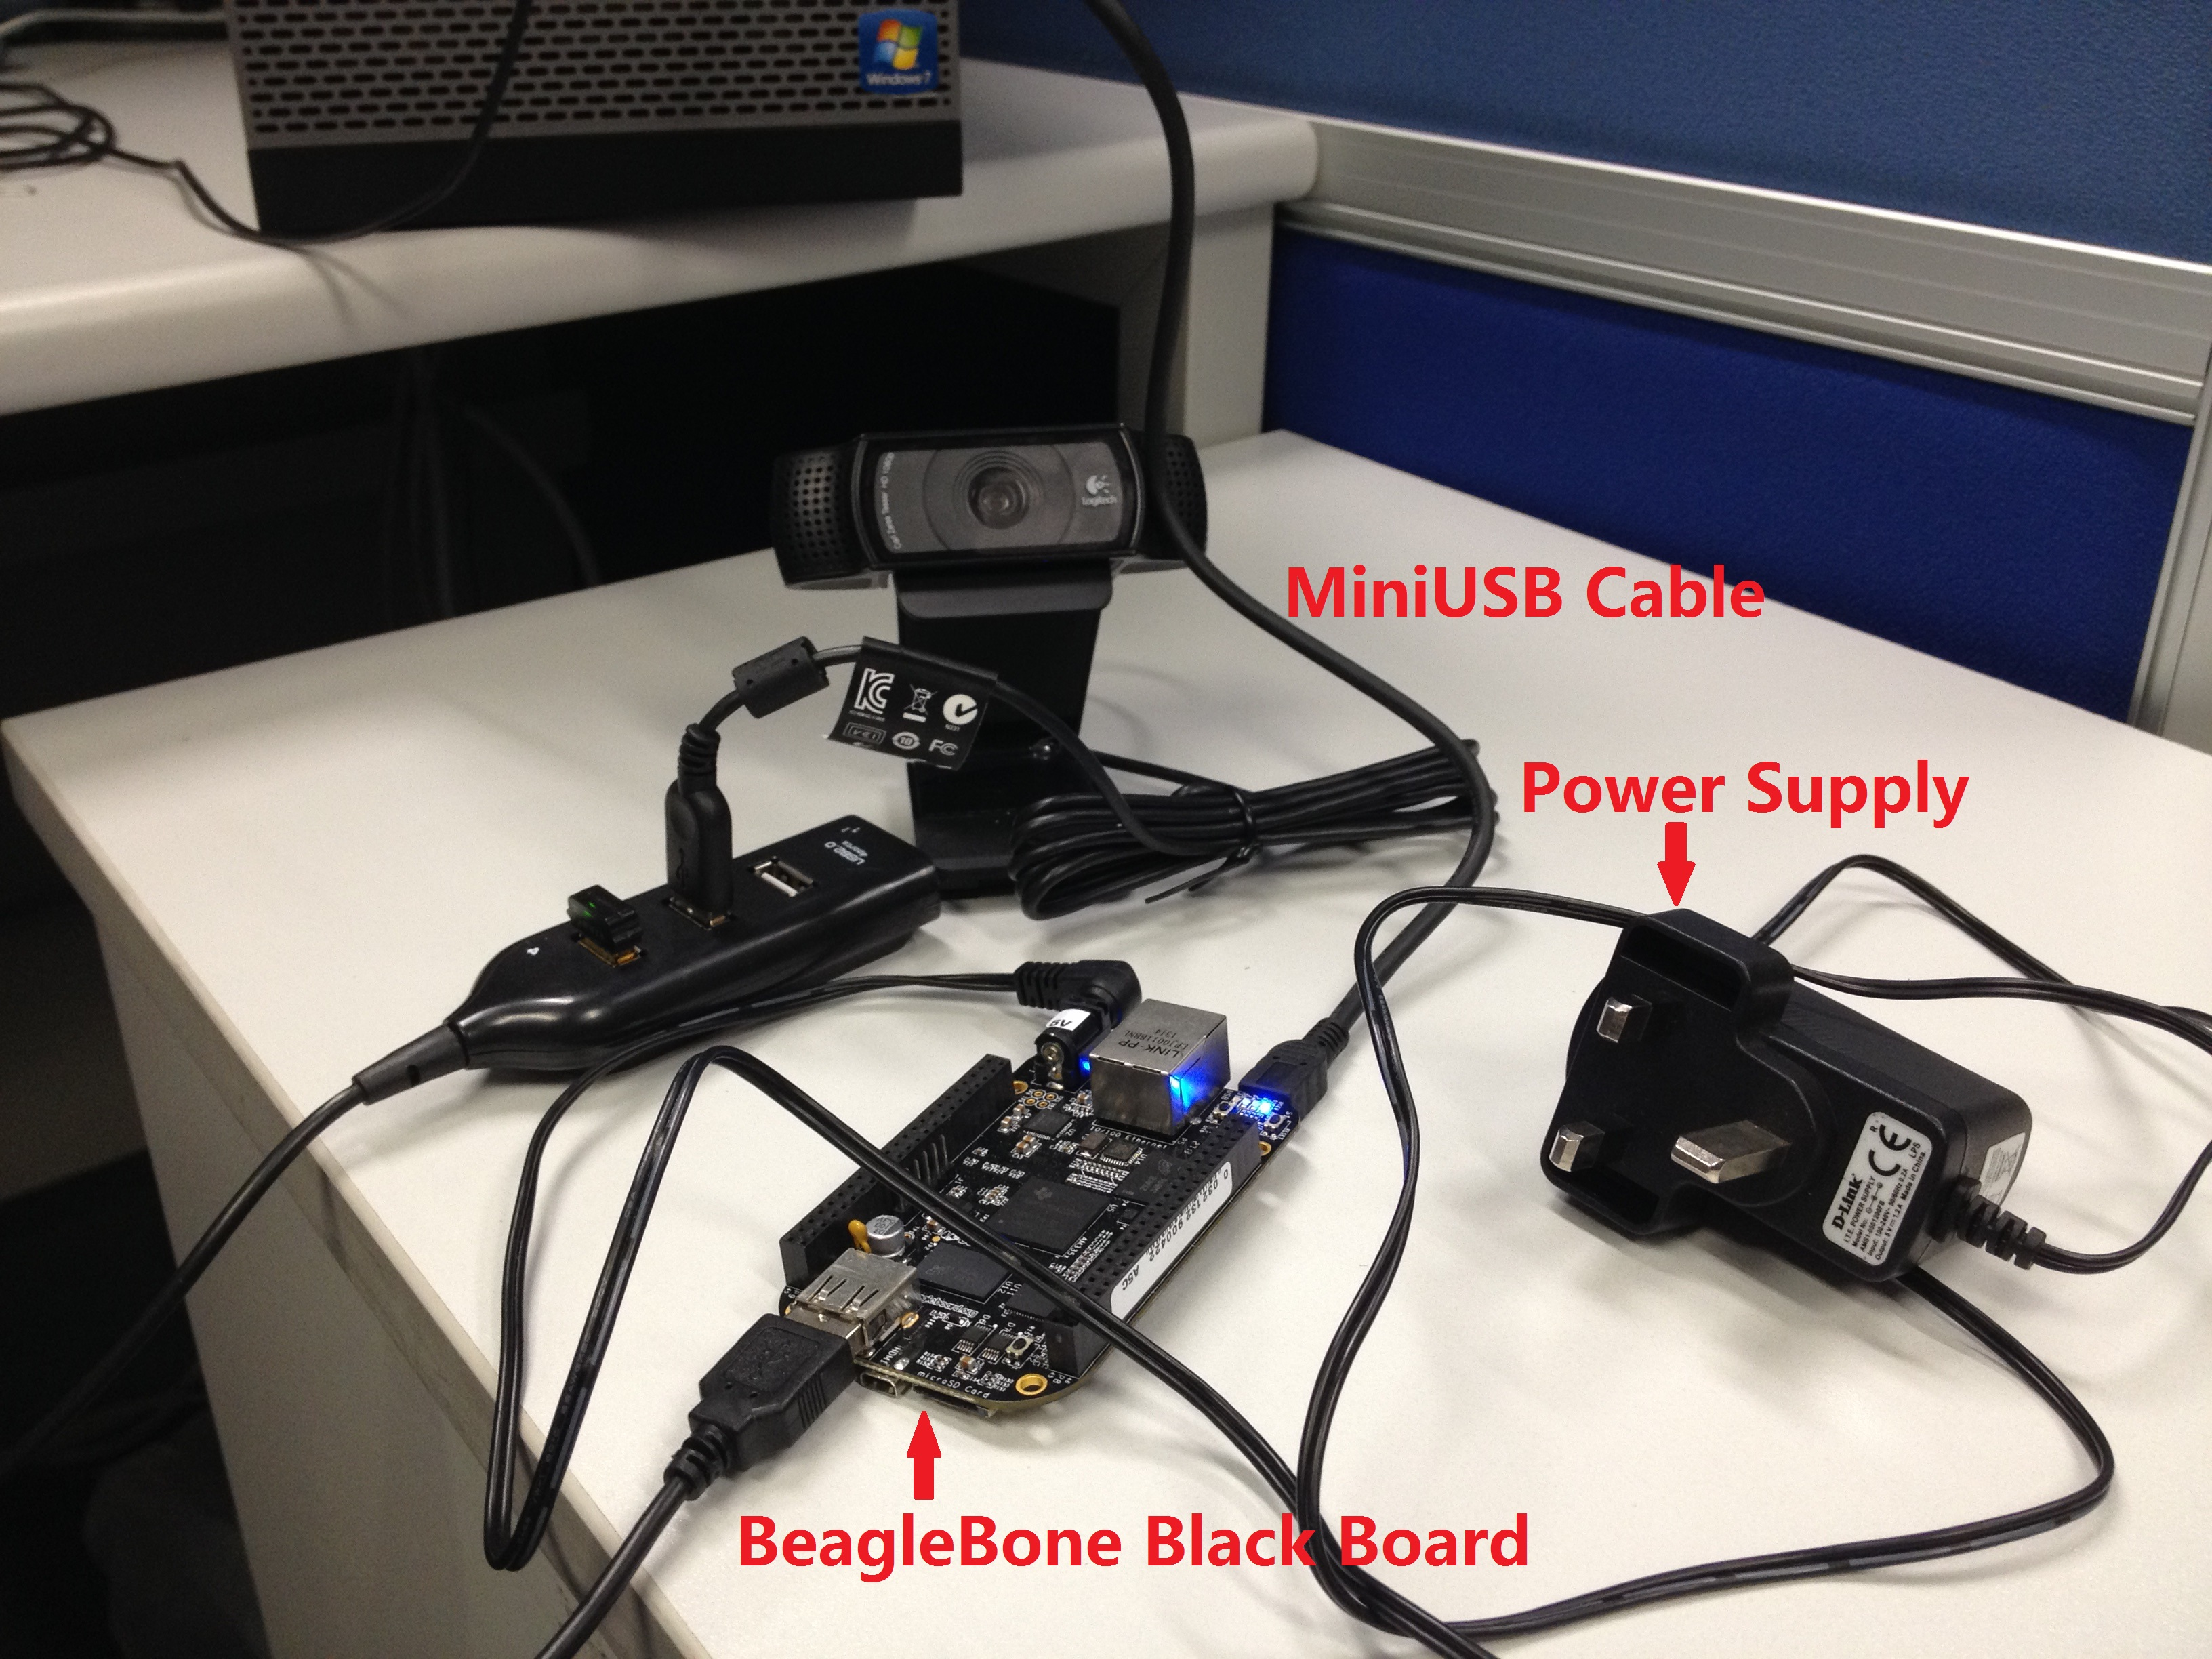
\includegraphics[width=4in]{./figs/hw2.jpg}
	\caption{Real view of hardware description.}
	\label{hw2}
\end{figure}

Both of the figures indicate the hardware setup details. First, the BBB board is connected to a PC using the MiniUSB Cable. Via the cable, the BBB board could not only receives a 5V/500mA power supply provided by PC's USB port, but also accesses to the Internet by setting up Windows ICS, in addition, users could operate Linux instructions through specific Windows-based software clients. Second, in case of unexpected system shutdown issue caused by current exceeding (current supply using MiniUSB Cable is set at a maximum of 500mA), an external power supply is used. Third, an USB Hub is connected to the onboard host USB port for expanding the port from one to four. Finally, the Logitech C920 webcam is connected to the USB Hub with its attached USB cable, together with a USB portable wireless adapter. Note that in this project, the BBB board could have an alternative way to access the Internet: getting access to a WiFi or a Hotspot connection via the wireless adapter; and the system could have two different IP address for Ethernet and wireless connection, respectively.


% % % % % % % % % % % % % % % % % % % % % % % % % % % % % % % % %
% % % % % % % % % % % % % % % % % % % % % % % % % % % % % % % % %
\section{Software Description and Implementation}\label{SfDes}
\begin{figure}[ht]
	\centering
	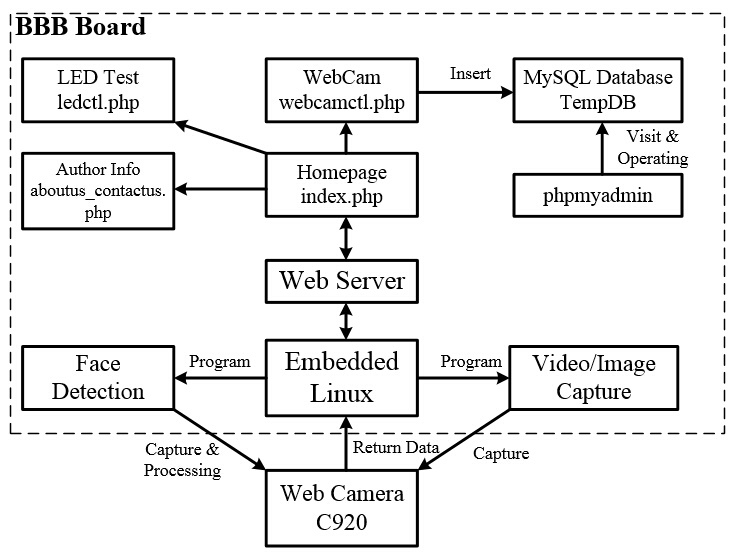
\includegraphics[width=6in]{./figs/sw1.jpg}
	\caption{Block diagram of software description.}
	\label{sw1}
\end{figure}

In this project, the software implementation includes installation, configuration as well as application of embedded OS, Web server, PHP, and MySQL; setup and website-based control of onboard LEDs and the C920 Web Camera. Fig.\ref{sw1} provides a block diagram of software description.

	\subsection{Operating System Installation and Configuration}\label{Sys}
	In our implementation, we install Ubuntu Trusty 14.04 on BBB. This image uses the Ubuntu 14.04 core filesystem from Ubuntu with the minimal meta package applied. The kernel is compiled from the mainline Linux kernel git repository. The result is an easy-to-install and stable Linux image that works well with the BBB boards.

First, OS binaries ``ubuntu-trusty-14.04-rootfs-3.14.4.1-bone-armhf.com.tar.xz" can be downloaded from \textcolor{blue}{\textit{\url{http://www.armhf.com/boards/beaglebone-black/}}}; After uncompressing this file, we can get the Ubuntu Trusty 14.04 image as shown in Fig.\ref{osimage}. Next, this image should be burn into a microSD card such that we can install Ubuntu 14.04 onto BBB. One way of doing this task is by utilising Win32DiskImager, which is a powerful tool automatically creating a OS boot disk and available at \textcolor{blue}{\textit{\url{http://sourceforge.net/projects/win32diskimager/files/latest/download}}}. In Fig.\ref{win32diskimager}, Win32DiskImager is starting to write Ubuntu.img to the microSD card, as presented by `device' F:. Please refer to the getting started page on the BeagleBone official website \cite{startBB} to find more details on the OS installation

\begin{figure}[htb]
	\centering
	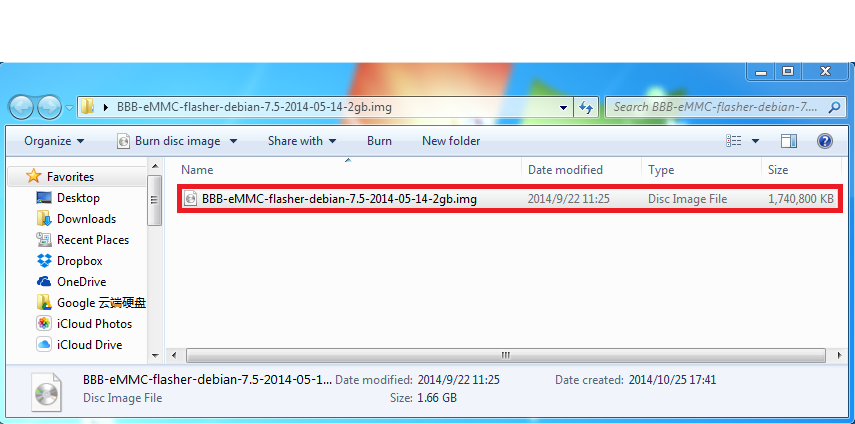
\includegraphics[width=4in]{./figs/osimage.PNG}
	\caption{Ubuntu Trusty 14.04 Image.}
	\label{osimage}
\end{figure}

\begin{figure}[htb]
	\centering
    \subfigure[MicroSD card.]{
       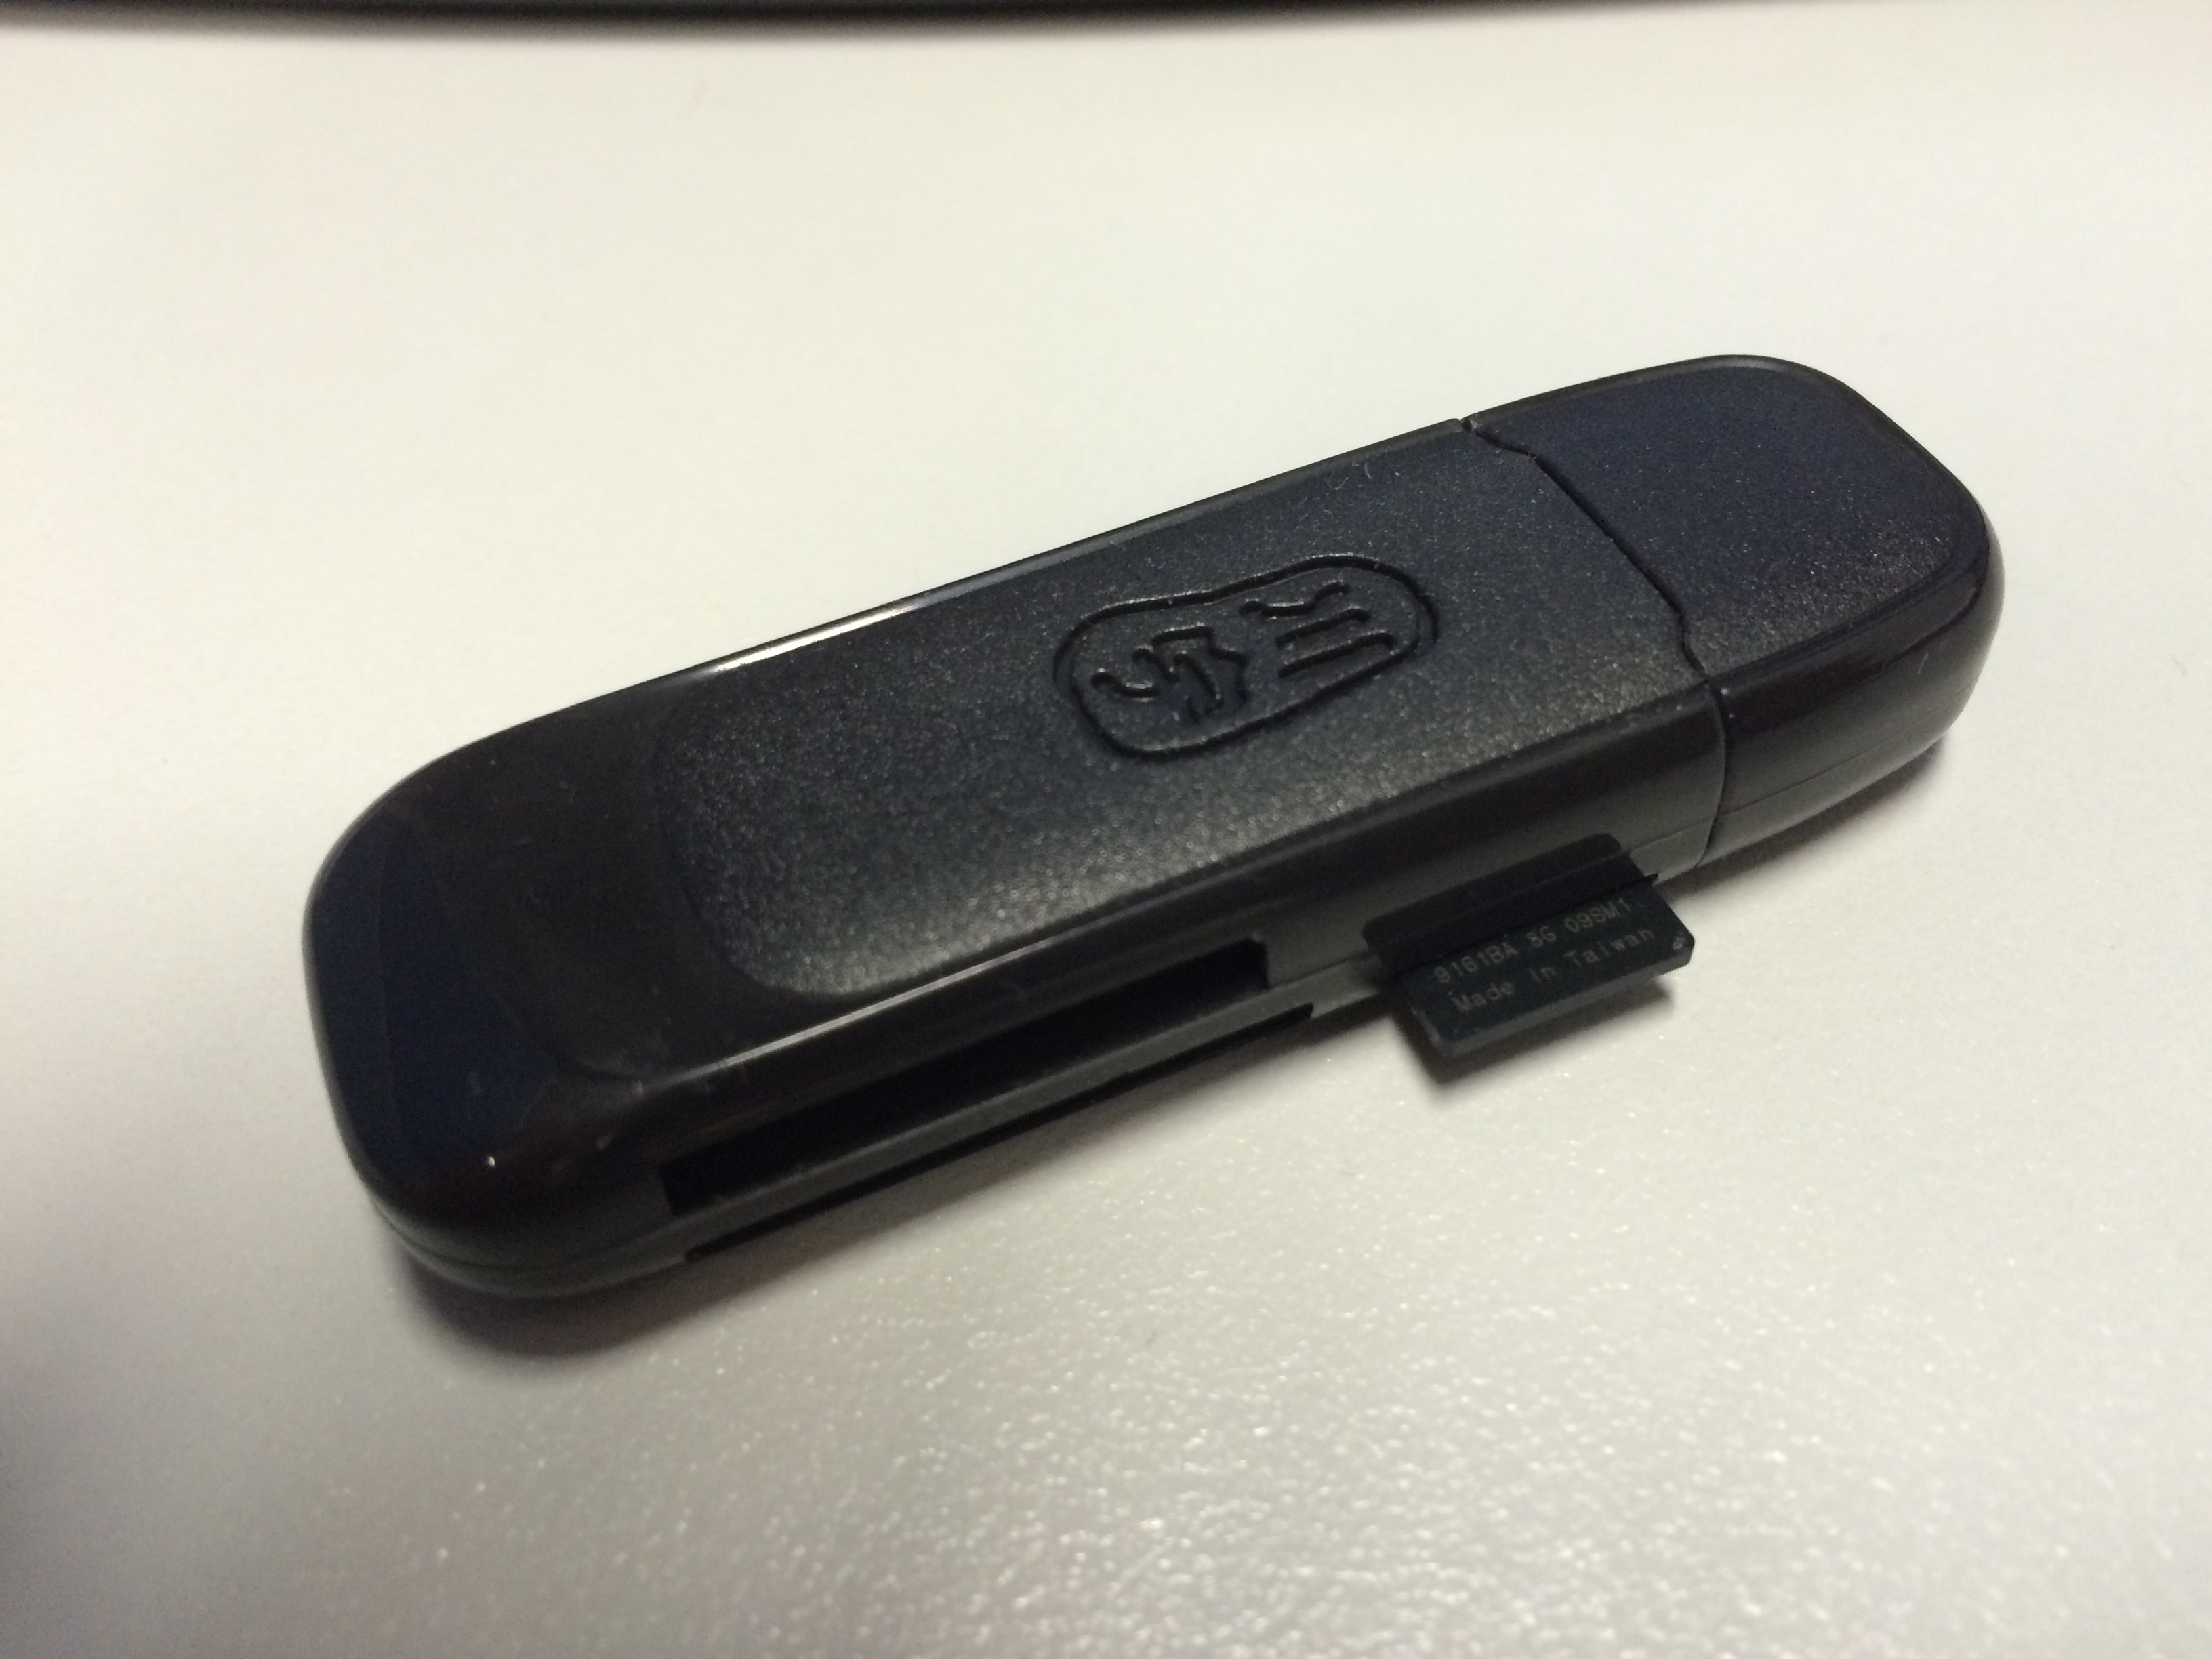
\includegraphics[width=2in]{./figs/microsd.JPG}
       \label{microsd}
     }
    \subfigure[Win32DiskImager]{
       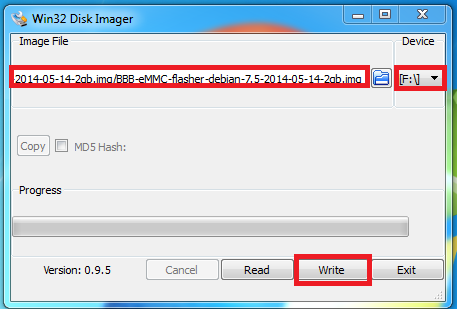
\includegraphics[width=2.5in]{./figs/win32diskimager.PNG}
       \label{win32diskimager}
     }
     \caption{Creating A Ubuntu bootable image on microSD card.}
     \end{figure}

When the microSD Card is now ready to boot, we insert it into BBB board, hold down the USER/BOOT button (in our board, it is S3 button.) and apply power, either by the USB cable or 5V adapter. However, it is strongly recommended to plug the 5V adapter in all the time because power adapter can provide more stable voltage than USB cable and thus it is less likely to have unexpected problems caused by power cutoff or insufficient.

Keep holding down the button until  the bank of 4 LED's light up for a few seconds and now release the button.
It will take anywhere from 30-45 minutes to flash the image onto the on-board chip. Once it's done, the bank of 4 LED's to the right of the Ethernet will all stay lit up at the same time. We can then power down your BBB \cite{flashBB}. One important thing worth mentioning is that after finishing this step, we do not need microSD card installation anymore --- you can plug it out and whenever you power the board again, Ubuntu is able to automatically boot from MMC, the inner storage component on chip.
	
\subsection{Wireless Adapter Configuration}\label{Wireless}
Once the OS is successfully set up on board, it becomes critical to have Internet access --- We need to install extra system utilities or download third-party libraries to support this project. So in this section, we detail how to setup a WiFi connection for BBB.

To begin with, we must connect the components needed into BBB: wireless network adapter, USB hub and miniUSB cable (See Fig.\ref{WiFi}). The wireless network adapter is the key for Internet connectivity. Besides this adapter, a webcam is also required by this project but we only have one USB port for them.  We therefore use a USB hub to install both components. We also need a miniUSB cable to connect BBB to the host PC such that we can remote control BBB through host PC's keyboard. Or to be more precise, we start a SSH connection to BBB through this cable.

\begin{figure}[htb]
	\centering
    \subfigure[Wireless Network Adapter]{
       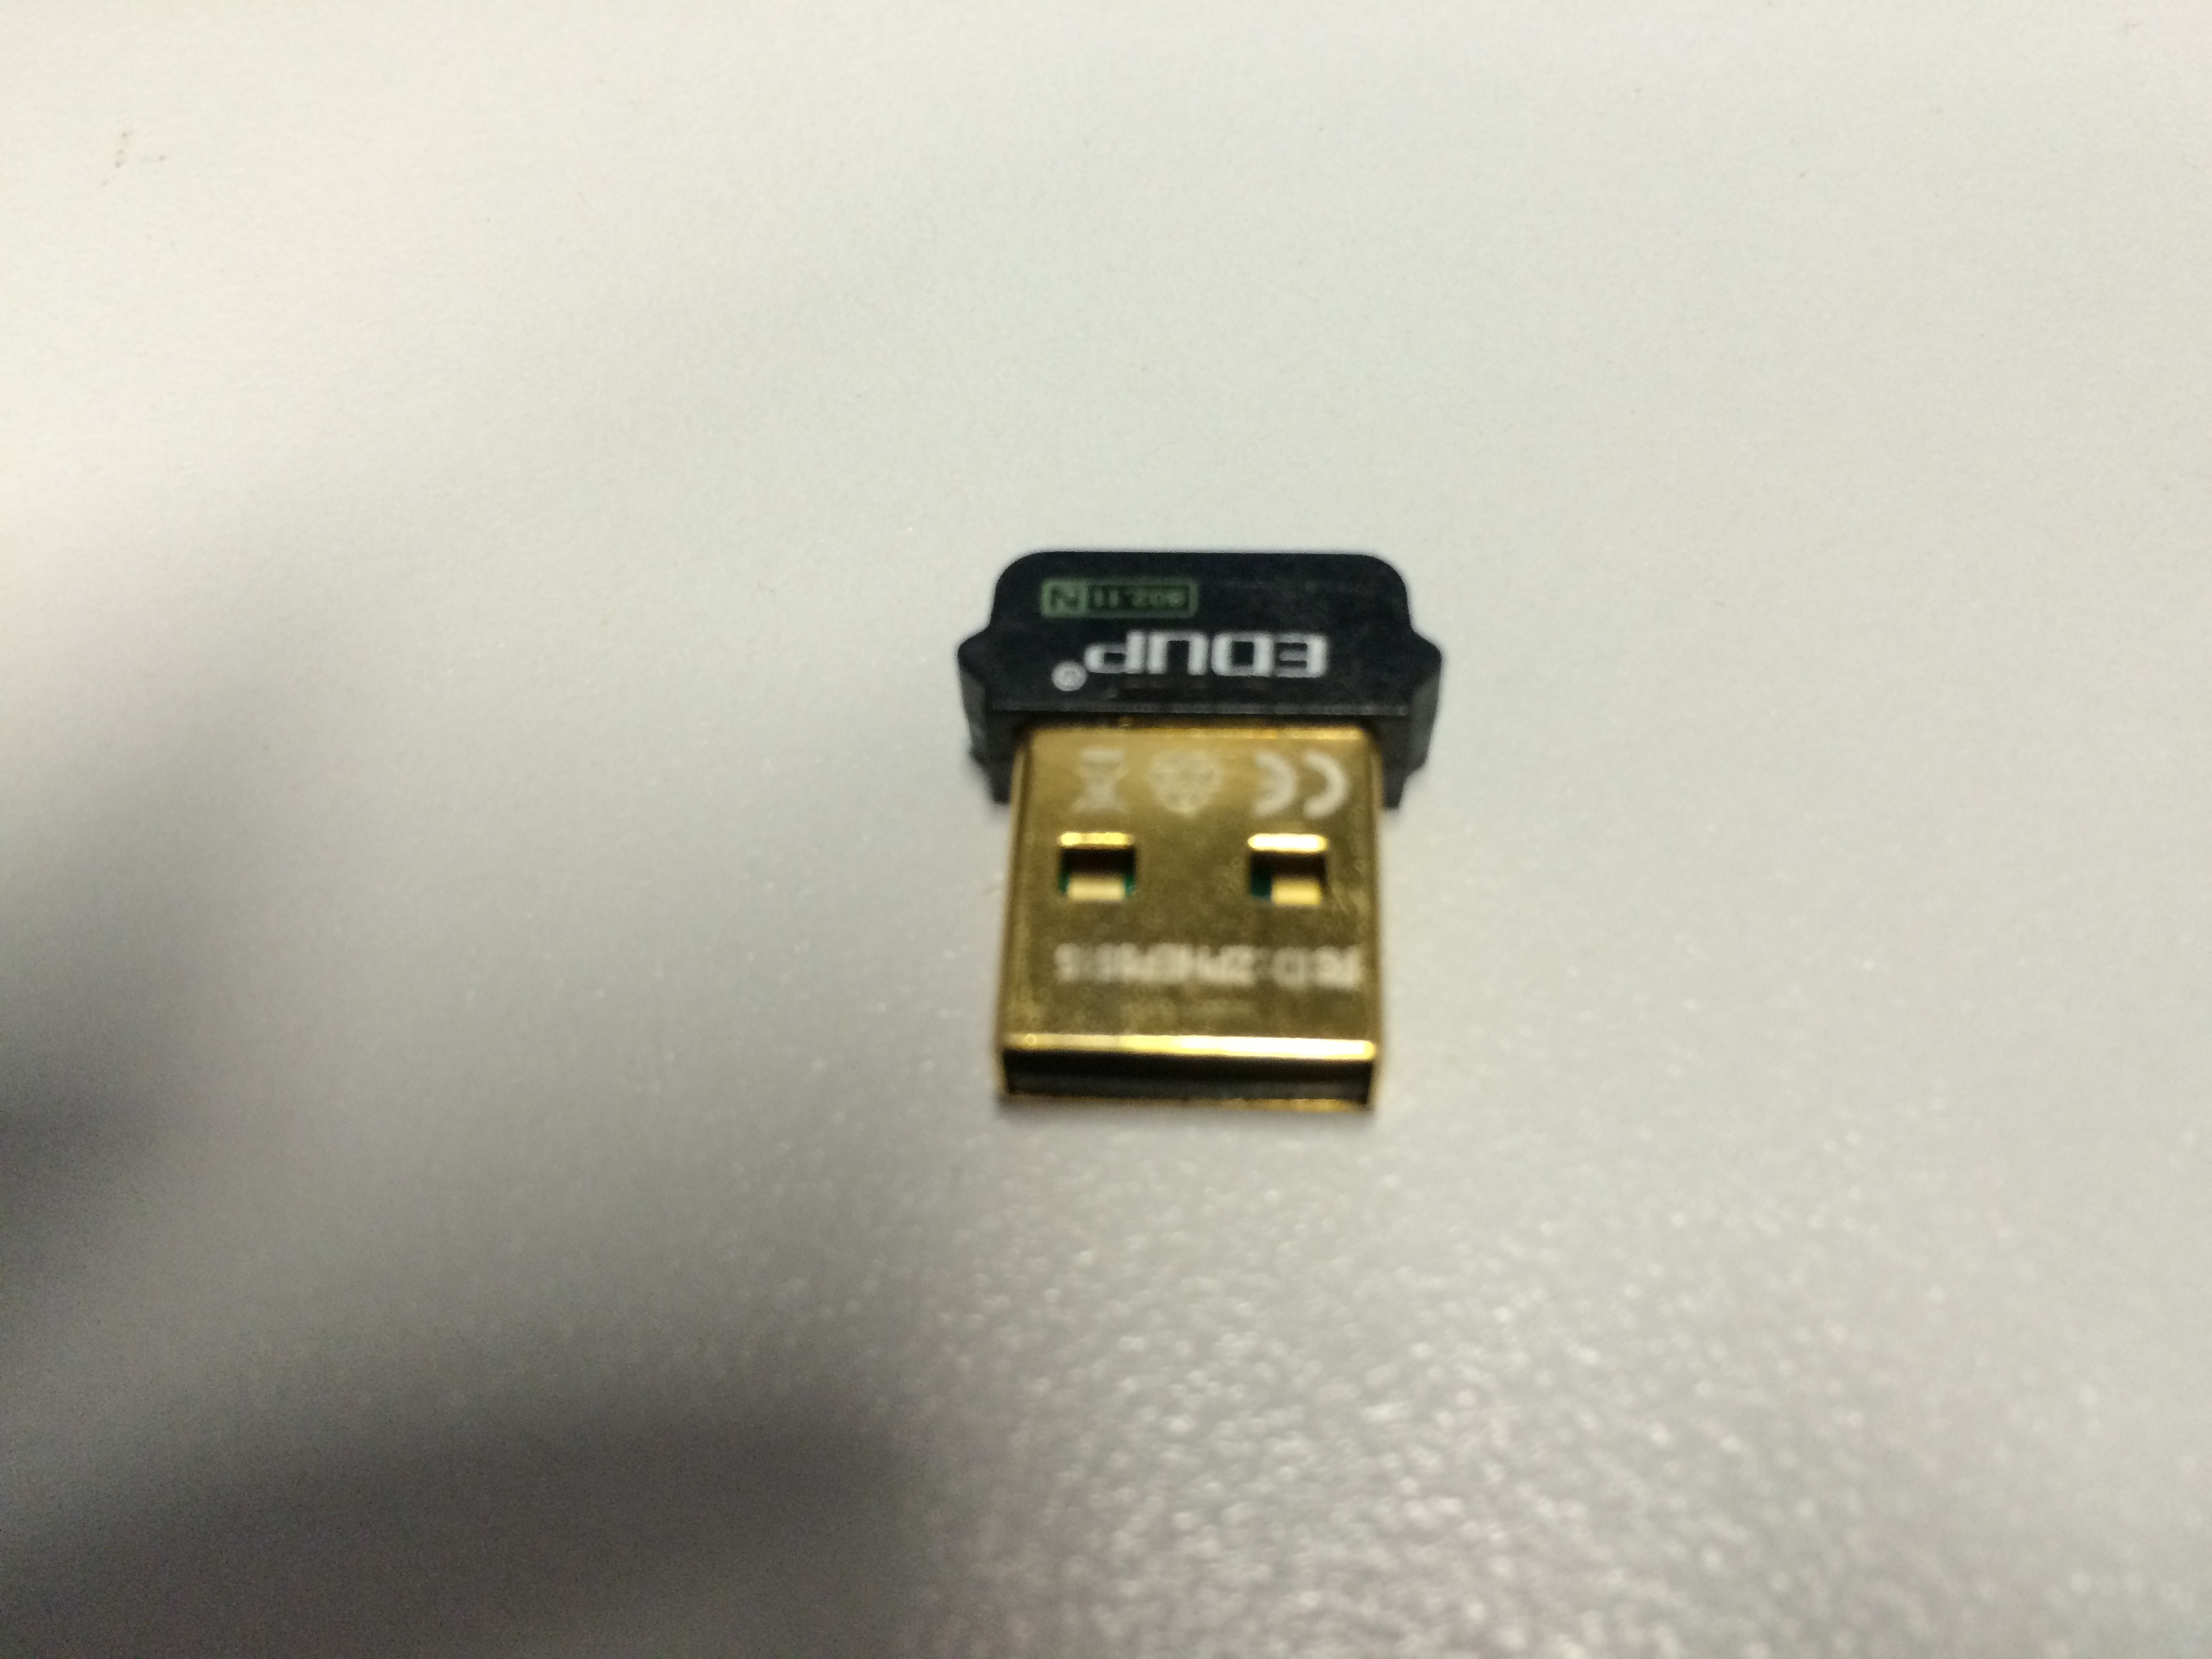
\includegraphics[width=2in]{./figs/wifiadapter.JPG}
       \label{wifiadapter.JPG}
     }
    \subfigure[Usb Hub]{
       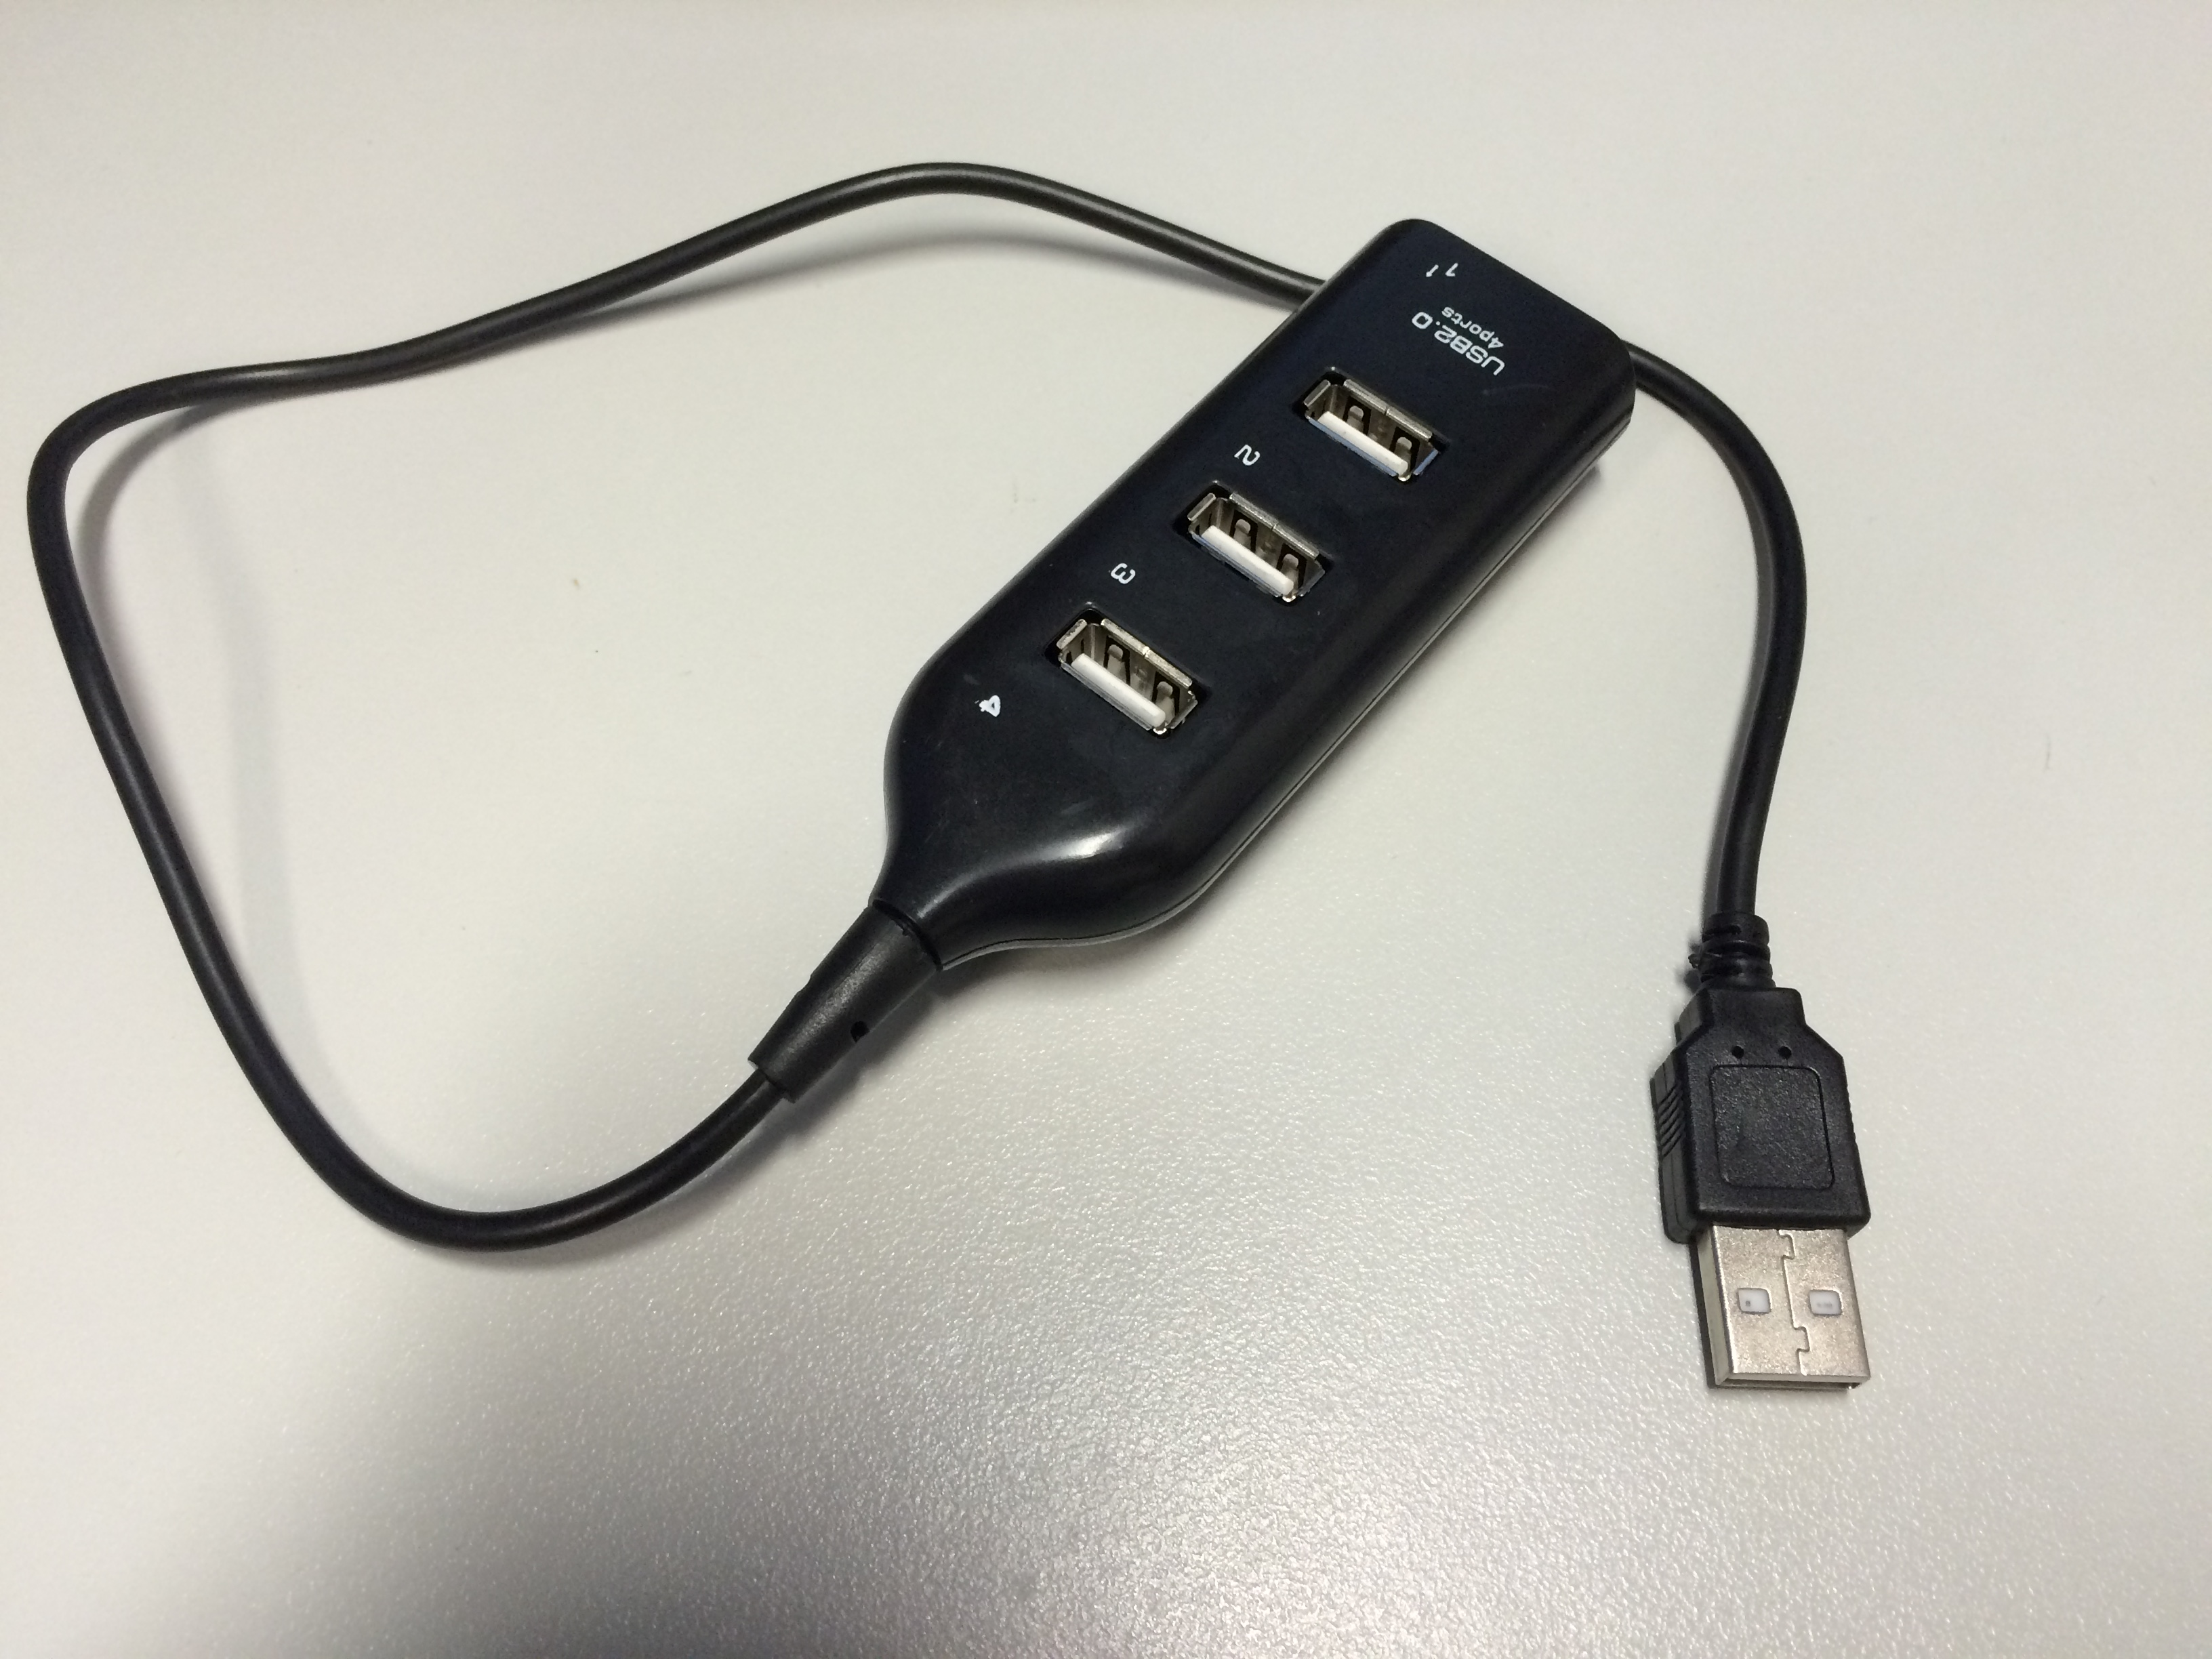
\includegraphics[width=2in]{./figs/usbhub.JPG}
       \label{usbhub.JPG}
     }
     \subfigure[MiniUSB Cable]{
       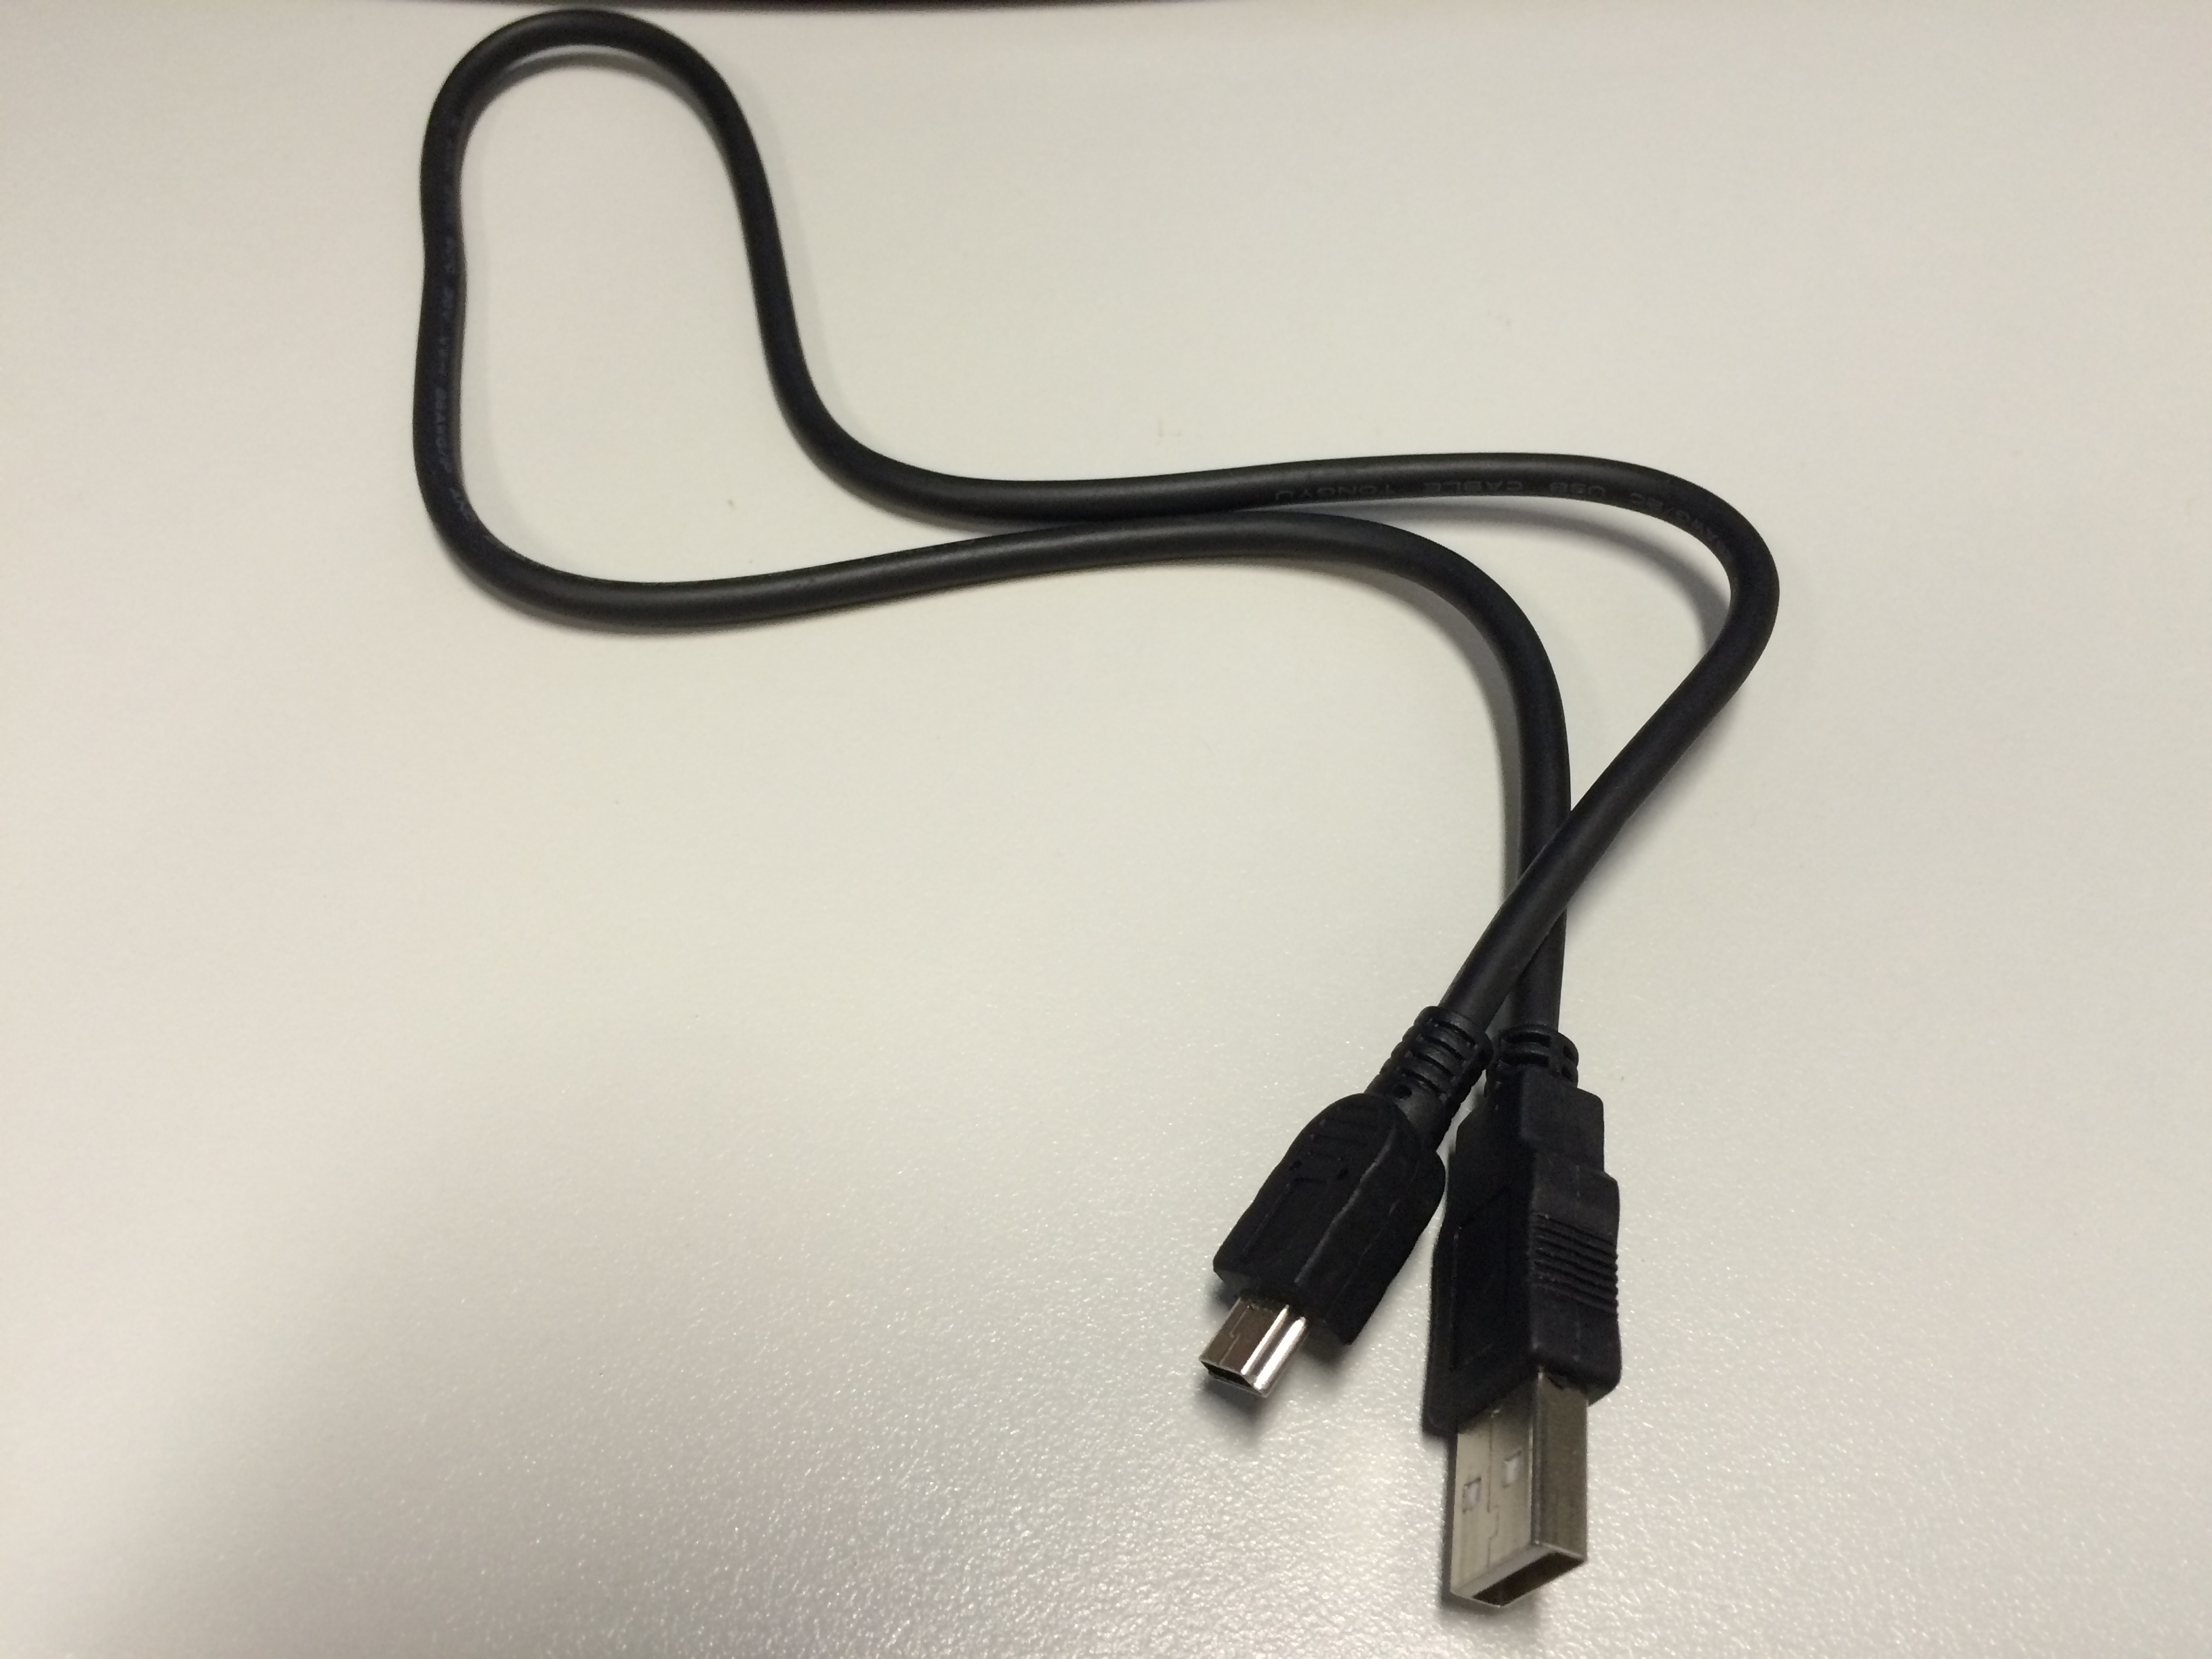
\includegraphics[width=2in]{./figs/miniusbcable.JPG}
       \label{miniusbcable.JPG}
     }
     \caption{Essential components for WiFi connection}
     \label{WiFi}
     \end{figure}

To establish SSH connection, we must log on BBB via SSH protocol and this could be done with the help of SSH tool. In fact, there are a variety of SSH GUI tools available for Windows. In this report, we take Secure Shell Client available on \textcolor{blue}{\textit{\url{http://mepopedia.com/forum/file.php?793,file=1103,filename=SSHSecureShellClient-3.2.9.exe,download=1}}}  as an example because this tool integrates scp command that allows us to transfer files between the host PC and the BBB freely.

When the wireless network adapter is plug into BBB and BBB itself is also connected to one USB port on our host PC, we open the Secure Shell Client and start a SSH connection from PC to BBB as shown in Fig.\ref{ssh}. Remember the default IP address for BBB is 192.168.7.2 and the default user account is `ubuntu' with password "temppwd".
\begin{figure}[htb]
	\centering

    \subfigure{
       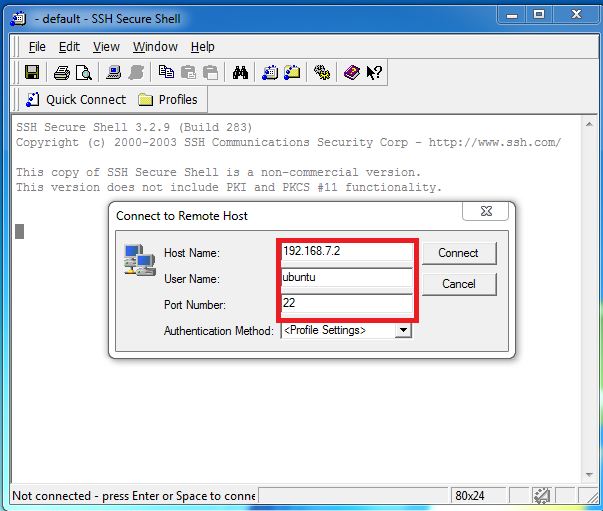
\includegraphics[width=2.5in]{./figs/ssh1.PNG}

     }
    \subfigure{
       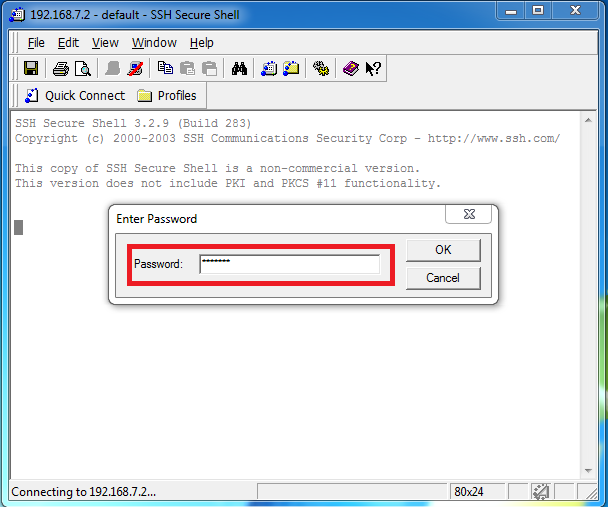
\includegraphics[width=2.5in]{./figs/ssh2.PNG}

     }
     \caption{SSH log on via Secure Shell Client for Windows.}\label{ssh}
     \end{figure}

\begin{figure}[htb]
	\centering
	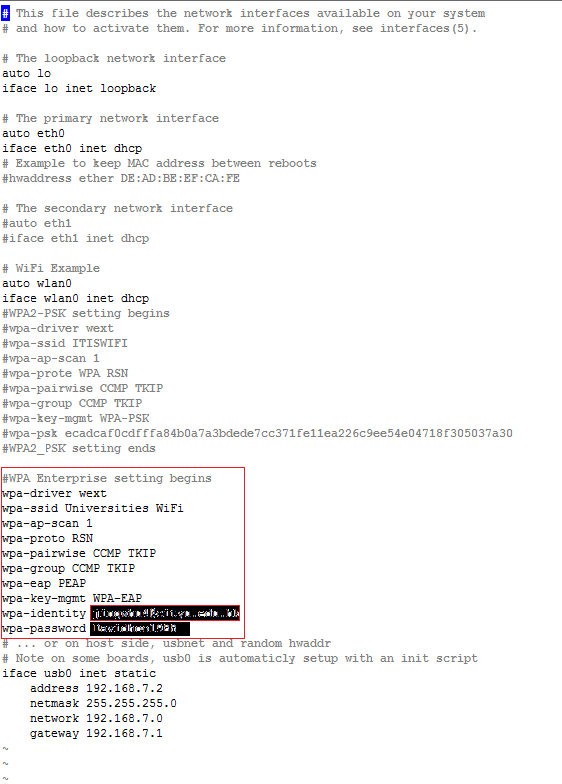
\includegraphics[width=4in]{./figs/wifi.PNG}
	\caption{Modify /ect/network/interfaces to establish a WiFi connection to access the Internet.}
	\label{wifi}
\end{figure}

Finally, we configure the WiFi setup by modifying the network configuration file located at /ect/network/interfaces.
In figure \ref{wifi} we present the changes that have been made marked in red box. The idea of the is to connect to CityU Campus WiFi network --- "Universities WiFi" with the student EID and password. For safety reason, the EID and password are wiped out and readers can use their own account to fill in.



To make the modifications into effect, we type in "ifconfig wlan0 down $\&\&$ ifconfig wlan0 up" from Secure Shell Client to restart the wirless adapter. Then we type in $ping www.google.com.hk$ to test whether the WiFi connection is functioning. Fig.\ref{ping} shows that the network setup is correct with all 4 transmitted packets getting received.

\begin{figure}[htb]
	\centering
	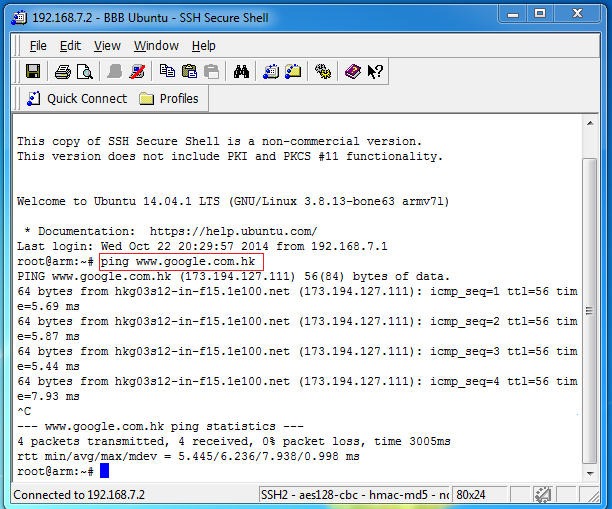
\includegraphics[width=5in]{./figs/ping.PNG}
	\caption{A successful ping to Google.}
	\label{ping}
\end{figure}

One last reminder is that we suggest to log in as `root' rather than `ubuntu'. This is primarily because `ubuntu' does have full access to all system resources and in many cases, you would get errors like `permission denied'. Just switch to `root' and all these annoying errors disappear.

\subsection{Web Server Setup}\label{Webser}
Apache together with PHP5 are used to establish the Web server. Apache can be installed on Ubuntu.
\begin{lstlisting}[language={bash}]
apt-get install apache2
\end{lstlisting}
Then, direct the browser to ``http://192.168.7.2" or ``http://*wireless IP address*", and the Apache placeholder page should appears: It Works! Note that the default document of placeholder page, or it can be called as homepage, can be found and edited at:
\begin{lstlisting}[language={bash}]
vi /var/www/index.php
\end{lstlisting}
	
In order to let Ubuntu can ``understand" PHP code, PHP5 and the Apache PHP5 modules must be installed. By installing both packages
\begin{lstlisting}[language={bash}]
apt-get install php5 libapache2-mod-php5
\end{lstlisting}
and restarting the Apache service
\begin{lstlisting}[language={bash}]
/etc/init.d/apache2 restart
\end{lstlisting}
PHP5 is configured and can be used for Web server developments. Please refer to \cite{Apache} for detailed Web server configuration and PHP testing examples.

After setting up the Web server, we could build our own main webpage by replacing the default $index.php$ file mentioned previously, with a modified one. Here, a CityU style webpage is designed and replaces the original one as the project main webpage, it can be accessed by typing either IP address of the board, see Fig.\ref{mainpage}. The template source code is provided by CityU of Hong Kong. All the sub pages' source code is stored under the path $/var/www/php/$, this indicates that visiting any sub websites, you should direct the browser to ``http://192.168.7.2/php/*source\ file\ name*".
\begin{figure}[htb]
	\centering
	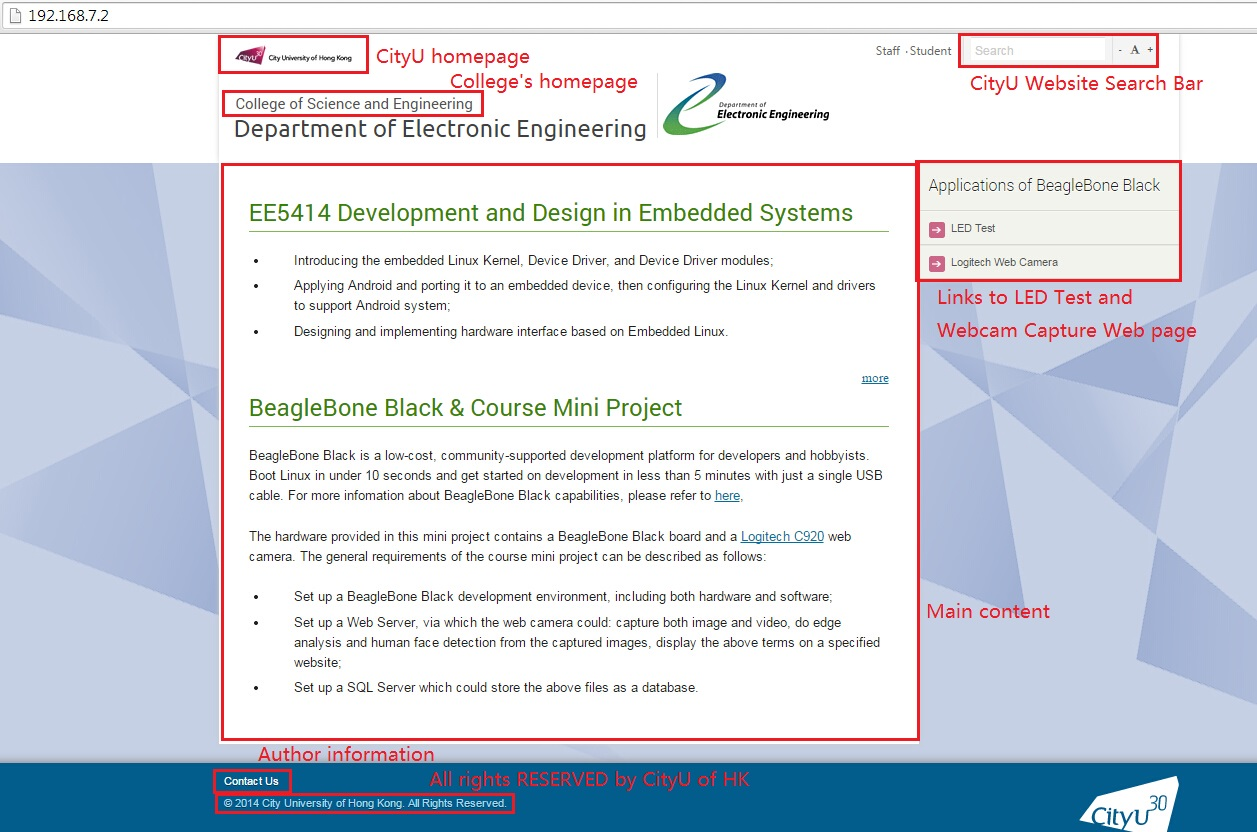
\includegraphics[width=6in]{./figs/mainpage.jpg}
	\caption{Project main webpage.}
	\label{mainpage}
\end{figure}
	
\subsection{LED Test}\label{Led}
The LED Test program is testing the four LED lights located near the Ethernet port and the Reset Button. In general, each LED light has two configuration files: one controls the trigger mode:
\begin{lstlisting}[language={bash}]
echo none > /sys/class/leds/beaglebone:green:usr?/trigger
\end{lstlisting}
``none" for passive mode and it can be changed to ``heartbeat" for blink mode; the other file controls the On/Off switch of the light:
\begin{lstlisting}[language={bash}]
echo 1 > /sys/class/leds/beaglebone:green:usr?/brightness
\end{lstlisting}
1 for light on, and 0 for light off. By default, some of the LEDs are used to display information to users about what is going on. So if the states those LEDs changes, they will be quickly overwritten. That is the reason why the trigger mode must be set before the stage of light changes in passive mode. And for blink mode, only the first command affects. Note that character ``$?$" in the above paths can be 0, 1, 2, and 3. Here gives the example of LED\_0 control shell script file.
\begin{lstlisting}[language={bash}]
#!/bin/bash
case "$1" in
'on')
echo "LED_0 is turned on"
sudo bash -c "echo none > /sys/class/leds/beaglebone:green:usr0/trigger"
sudo bash -c "echo 1 >    /sys/class/leds/beaglebone:green:usr0/brightness"
;;
'off')
echo "LED_0 is turned off"
sudo bash -c "echo none > /sys/class/leds/beaglebone:green:usr0/trigger"
sudo bash -c "echo 0 >    /sys/class/leds/beaglebone:green:usr0/brightness"
;;
'heartbeat')
echo "LED_0 is blinking"
sudo bash -c "echo heartbeat > /sys/class/leds/beaglebone:green:usr0/trigger"
;;
esac
\end{lstlisting}
Similarly, the shell script can be written to control all four LEDs. An example of the control command:
\begin{lstlisting}[language={bash}]
/var/www/LED/ledctl.sh on off on heartbeat 
\end{lstlisting}
By calling this shell script in the $.php$ file,
\begin{lstlisting}[language={PHP}]
<?php
...
$cmd = `/bin/bash ../LED/ledctl.sh $status0 $status1 $status2 $status3`;
...
?>
\end{lstlisting}
the website based LED test can be implemented. See Fig.\ref{LEDTest}: Fig.\ref{LEDTest1} indicates LED\_0 and 2 are switched on, LED\_1 is switched off, and LED\_3 is blink mode.
\begin{figure}[ht]
	\centering
	
	\subfigure[]{
		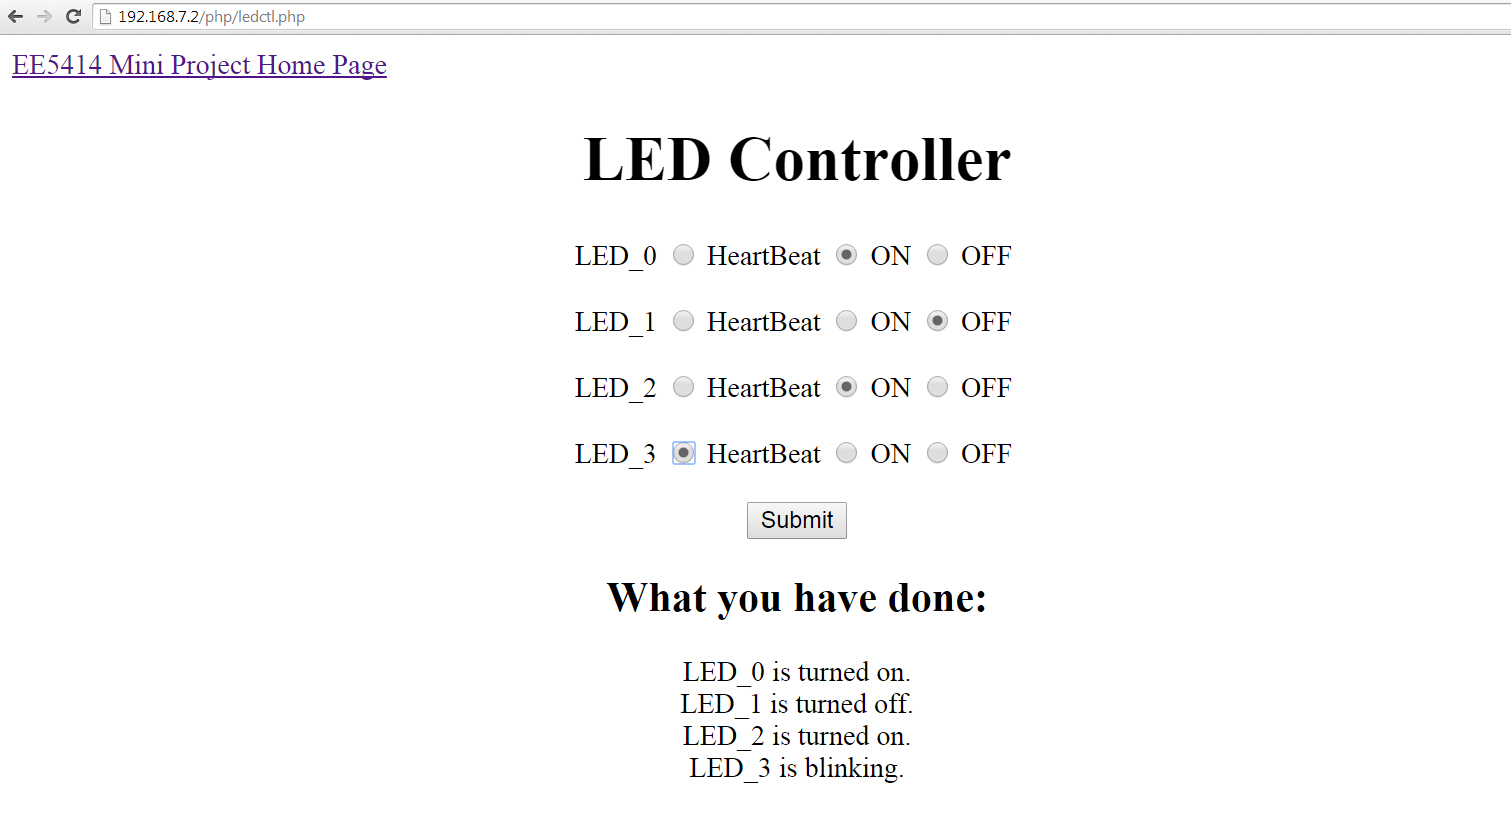
\includegraphics[width=5in]{./figs/LED1.jpg}\label{LEDTest1}		
	}
	\subfigure[]{
		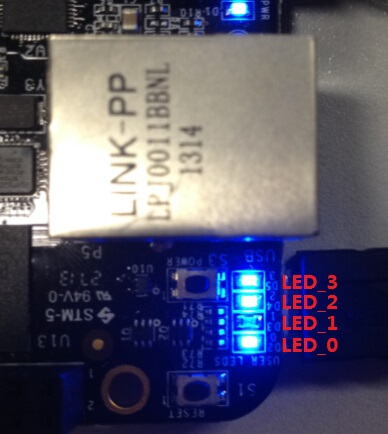
\includegraphics[width=2.5in]{./figs/LED2.jpg}\label{LEDTest2}		
	}
	\subfigure[]{
		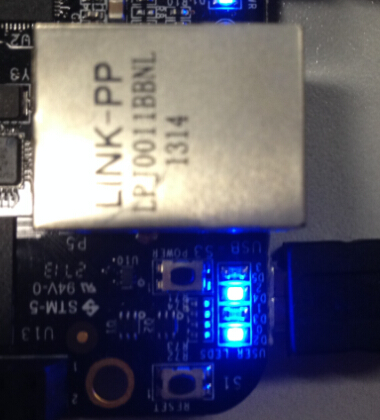
\includegraphics[width=2.5in]{./figs/LED3.jpg}\label{LEDTest3}		
	}
	\caption{Web based LED test.}\label{LEDTest}
\end{figure}

\subsection{Web Camera Configuration and Functioning}\label{Webcam}
In this subsection, a webcam controller is implemented on our Apache web server. A webcamctl.php file is coded for basic functions like photographing, video capturing and face detection. The corresponding web page can be accessed by typing "192.168.7.2/webcamctl.php" in the address bar of your web broswer if BBB is connected to the host PC.  A snapshot of this .php file and its web page is shown in Fig.\ref{webcam}.

\begin{figure}[htb]
	\centering

    \subfigure[/var/www/php/webcamctl.php]{
       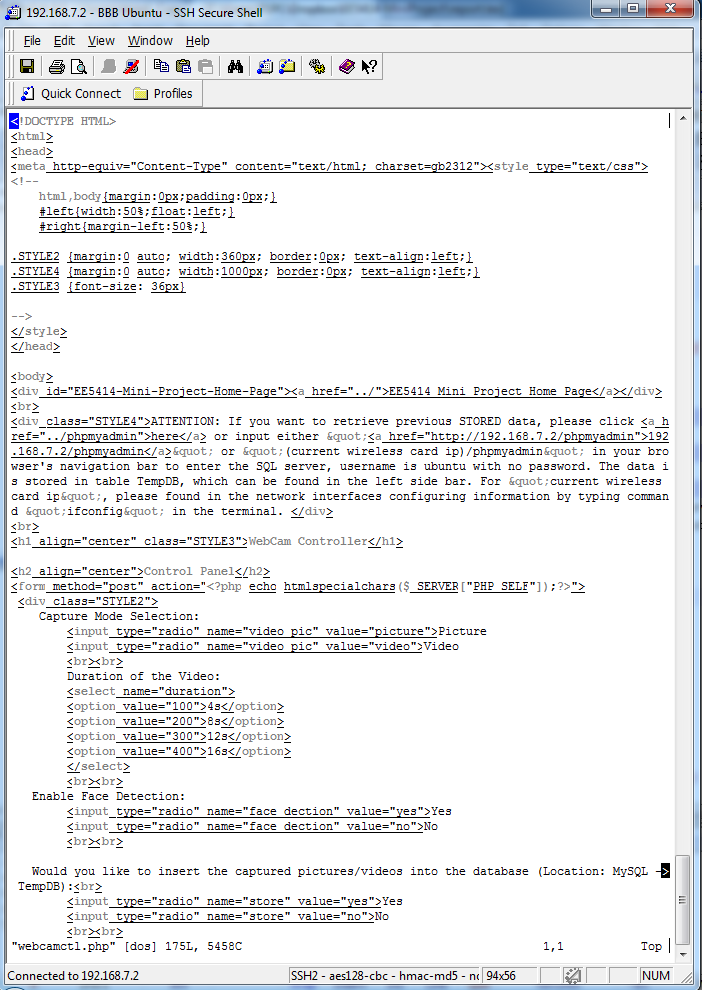
\includegraphics[width=3in]{./figs/webcam.PNG}

     }
    \subfigure[web page for webcam controller]{
       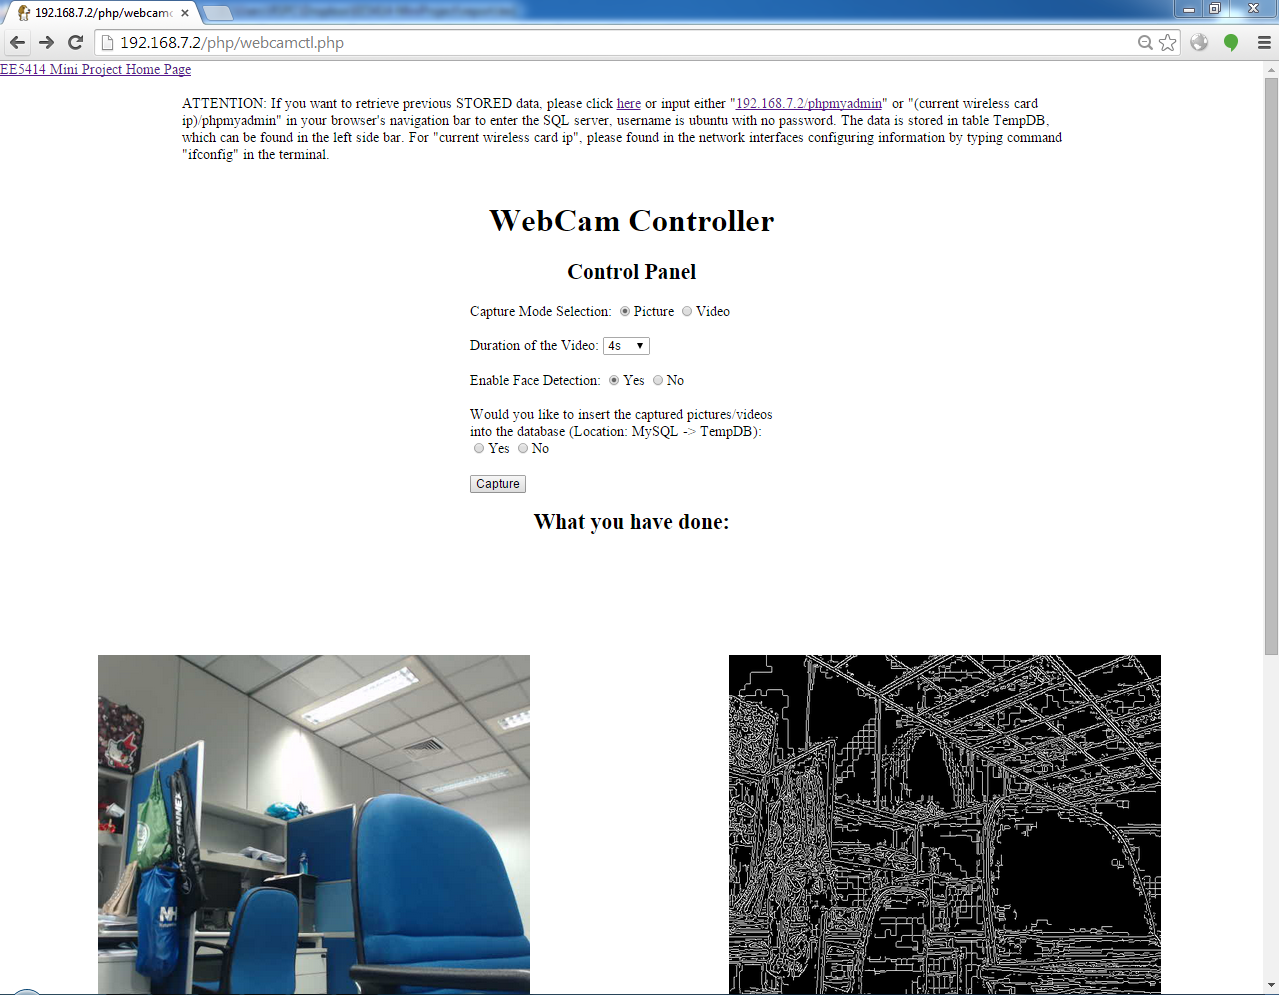
\includegraphics[width=3in]{./figs/webcam2.PNG}

     }
     \caption{PHP File Configuration and Web Page}\label{webcam}
     \end{figure}

It is suggested to use OpenCV library to achieve these functionalities because this library is cross-platform, which focuses mainly on real-time image processing and is free for use under the open source BSD license.
On top of this, OpenCV is pre-installed by default on our Ubuntu Trusty 14.04 operating system and thus it is not necessary to take pains learning how to immigrate OpenCV into BBB board. For photographing, it is optional to enable face detection function or not. Besides, it automatically detects the edge of this picture by using image edge detection method;  For video capturing, we also provide with 4 options for the capture duration: 4 seconds, 8 seconds, 12 seconds and 16 seconds.  We present below in Fig.\ref{webcamdemo} the demo of this work by detecting the author himself.
\begin{figure}[htb]
	\centering
	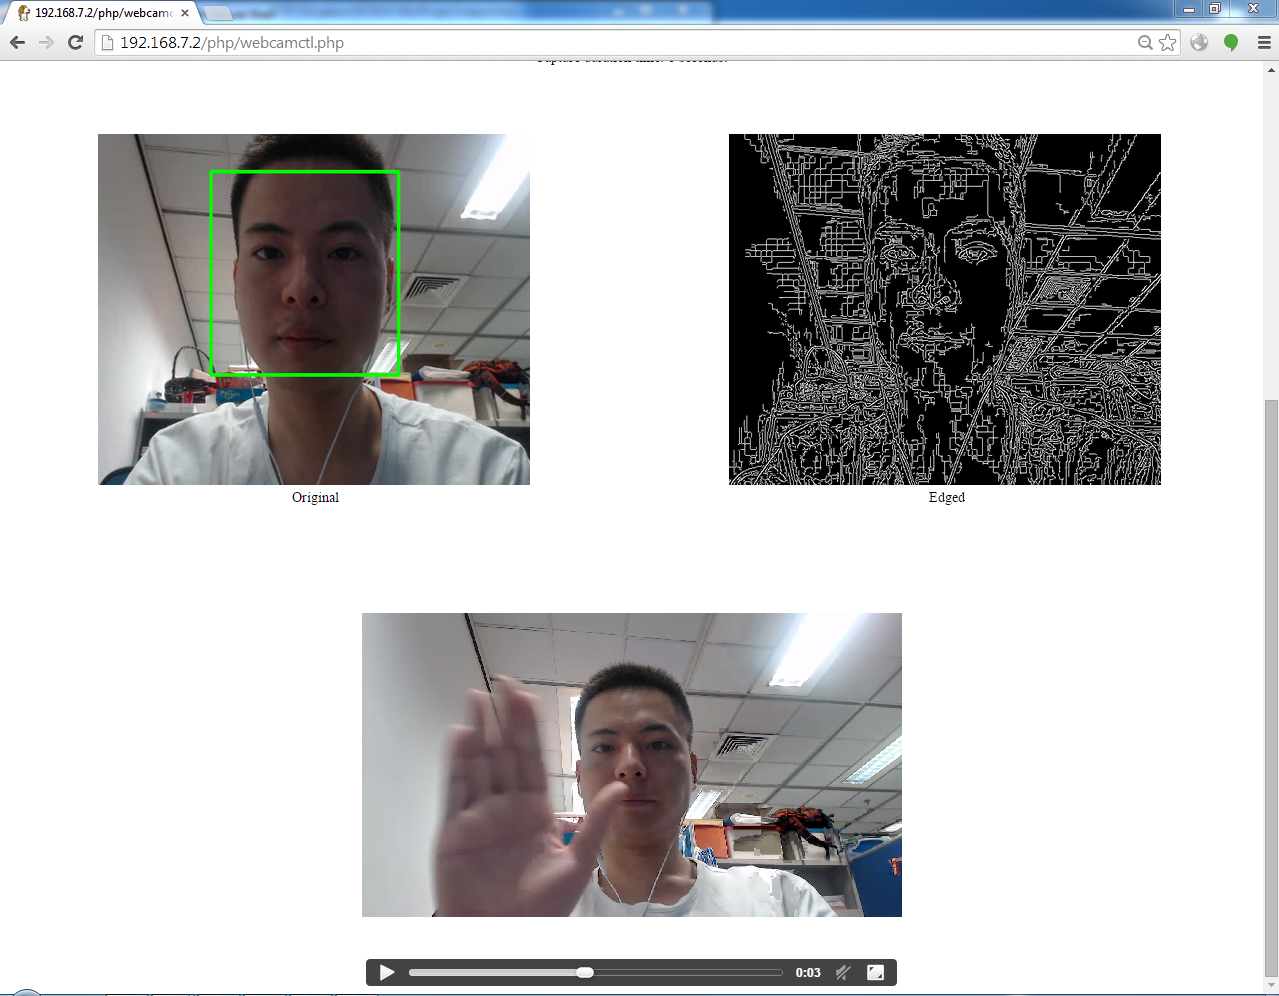
\includegraphics[width=4in]{./figs/webcam3.PNG}
	\caption{Demonstrate for the webcam controller}
	\label{webcamdemo}
\end{figure}

The details about the implementation of photographing and video capturing is introduced by Derek Molloy in his personal website \cite{molloy}. Please refer to \textcolor{blue}{\textit{\url{http://derekmolloy.ie/beaglebone/beaglebone-video-capture-and-image-processing-on-embedded-linux-using-opencv/}}} and \textcolor{blue}{\textit{\url{http://stackoverflow.com/questions/20757147/opencv-and-cdetect-face-in-image}}} for more details.


\subsection{SQL Server Setup and Application}\label{Sql}

	
\section{Conclusions}\label{Con}

% % % % % % % % % % % % % % % % % % % % % % % % % % % % % % % % %
% % % % % % % % % % % % % % % % % % % % % % % % % % % % % % % % %
\section*{Acknowledgment}
We would like to thank our colleague Sean Yang  for his kindly help with the WiFi setup on BBB board.

\bibliographystyle{plain}
\bibliography{bibfile}

\end{document}



%\bibliographystyle{plain}
%\bibliography{source}

